\chapter{La dissolution des solides ioniques et moléculaires}\label{ch:g11:dissolution}

Une pincée de sel remuée dans l'eau disparaît en quelques secondes~; la
même pincée remuée dans de l'huile de cuisine reste au fond du verre,
inchangée, aussi longtemps qu'on veut bien la regarder. Une poêle grasse
rincée sous le robinet reste grasse~; une goutte de liquide vaisselle, et
la graisse se détache. Qu'est-ce qui décide si une substance \omterm{def:g2:mixing-and-dissolving:dissolve}{se dissout}
dans un liquide~? La réponse se trouve dans les \omterm{def:g11:polarity-and-cohesion:polar-bond}{charges partielles} et
les forces entre particules du chapitre précédent.

\begin{recall}
La \omterm{def:g6:solutions-and-solubility:solubility}{solubilité}~; les liquides \omterm{def:g6:solutions-and-solubility:miscible}{miscibles} et \omterm{def:g6:solutions-and-solubility:miscible}{non miscibles}
(\cref{ch:g6:solutions-and-solubility}). Un \omterm{def:g9:ions:ionic-compound}{composé ionique} est formé de
\omterm{def:g9:ions:ion}{cations} et d'\omterm{def:g9:ions:ion}{anions} en proportions qui le rendent neutre
(\cref{ch:g9:ions}). Les \omterm{def:g11:polarity-and-cohesion:polar-molecule}{molécules polaires} et apolaires, les \omterm{def:g11:polarity-and-cohesion:hydrogen-bond}{liaisons
hydrogène}, les \omterm{def:g11:polarity-and-cohesion:van-der-waals}{interactions de van der Waals}
(\cref{ch:g11:polarity-and-cohesion}). L'\omterm{def:g10:chemical-species:extraction}{extraction liquide--liquide}
(\cref{ch:g10:chemical-species}). La \omterm{def:g10:concentration-and-dilution:molar-concentration}{concentration molaire}
(\cref{ch:g10:concentration-and-dilution}).
\end{recall}

\section{La dissolution d'un solide ionique}

Dans un cristal de chlorure de sodium, chaque \omterm{def:g9:ions:ion}{ion} sodium \ce{Na+} est
entouré d'\omterm{def:g9:ions:ion}{ions} chlorure \ce{Cl-} et chaque \omterm{def:g9:ions:ion}{ion} chlorure d'\omterm{def:g9:ions:ion}{ions} sodium,
tous retenus par l'attraction entre charges opposées. Les \omterm{def:g7:atoms-and-molecules:molecule}{molécules}
d'eau, polaires, sont attirées par ces charges~: leur côté oxygène
($\delta^-$) se tourne vers les \omterm{def:g9:ions:ion}{cations}, leur côté hydrogène
($\delta^+$) vers les \omterm{def:g9:ions:ion}{anions}.

\begin{definition}[Dissociation]\label{def:g11:dissolution:dissociation}
La \emph{dissociation}\index{dissociation} d'un solide ionique dans un
\omterm{def:g6:solutions-and-solubility:solute}{solvant} est la séparation de ses \omterm{def:g9:ions:ion}{ions} les uns des autres~: ils quittent
le cristal et s'éloignent les uns des autres dans la solution.
\end{definition}

\begin{definition}[Solvatation, hydratation]\label{def:g11:dissolution:solvation}
La \emph{solvatation}\index{solvatation} d'une particule dissoute est le
fait qu'elle s'entoure de \omterm{def:g7:atoms-and-molecules:molecule}{molécules} de \omterm{def:g6:solutions-and-solubility:solute}{solvant}, retenues par des
attractions~; dans l'eau, on parle d'\emph{hydratation}\index{hydratation}.
Le symbole (aq) placé après une formule signifie «~hydraté~».
\end{definition}

\begin{proposition}[Les trois étapes de la dissolution]\label{prop:g11:dissolution:stages}
Un solide ionique \omterm{def:g2:mixing-and-dissolving:dissolve}{se dissout} dans l'eau en trois étapes simultanées~:
les \omterm{def:g9:ions:ion}{ions} sont arrachés au cristal (\omterm{def:g11:dissolution:dissociation}{dissociation}), entourés de \omterm{def:g7:atoms-and-molecules:molecule}{molécules}
d'eau (\omterm{def:g11:dissolution:solvation}{hydratation}), et répartis dans toute la solution (dispersion).
Pour le chlorure de sodium,
\[
  \ce{NaCl(s) -> Na+(aq) + Cl-(aq)} .
\]
\end{proposition}

\begin{proof}
Admis~: les attractions entre les \omterm{def:g9:ions:ion}{ions} et les \omterm{def:g7:atoms-and-molecules:molecule}{molécules} d'eau polaires,
additionnées, sont assez fortes pour remplacer celles qui unissent les
\omterm{def:g9:ions:ion}{ions} du cristal.
\end{proof}

\begin{omfigure}
\begin{tikzpicture}[font=\small]
  % the crystal edge: alternating ions
  \foreach \i in {0,1,2,3,4} \foreach \j in {0,1,2,3} {
    \pgfmathtruncatemacro\k{mod(\i+\j,2)}
    \ifnum\k=0
      \node[om atom, ball color=green!60!black, minimum size=6.4mm] at (0.8*\i,0.8*\j) {};
    \else
      \node[om atom, ball color=violet!70, minimum size=4.0mm] at (0.8*\i,0.8*\j) {};
    \fi
  }
  % a hydrated Na+ that has left: O towards the ion
  \begin{scope}[shift={(5.6,1.8)}]
    \node[om atom, ball color=violet!70, minimum size=4.0mm] (na) at (0,0) {};
    \node[font=\footnotesize] at (0,0) {};
    \foreach \a in {0,90,180,270} {
      \node[aO, minimum size=4.6mm] (o\a) at (\a:0.62) {};
      \node[aH, minimum size=3.2mm] (ha\a) at ($(\a:0.62)+(\a+52:0.42)$) {};
      \node[aH, minimum size=3.2mm] (hb\a) at ($(\a:0.62)+(\a-52:0.42)$) {};
      \begin{scope}[on background layer]
        \draw[bond, line width=1.2pt] (o\a.center) -- (ha\a.center);
        \draw[bond, line width=1.2pt] (o\a.center) -- (hb\a.center);
      \end{scope}
    }
    \node[anchor=north] at (0,-1.35) {\ce{Na+(aq)}};
  \end{scope}
  % a hydrated Cl- that has left: H towards the ion
  \begin{scope}[shift={(8.6,1.4)}]
    \node[om atom, ball color=green!60!black, minimum size=6.4mm] at (0,0) {};
    \foreach \a in {45,135,225,315} {
      \node[aH, minimum size=3.2mm] (h\a) at (\a:0.62) {};
      \node[aO, minimum size=4.6mm] (o\a) at (\a:1.0) {};
      \node[aH, minimum size=3.2mm] (k\a) at ($(\a:1.0)+(\a+75:0.42)$) {};
      \begin{scope}[on background layer]
        \draw[bond, line width=1.2pt] (o\a.center) -- (h\a.center);
        \draw[bond, line width=1.2pt] (o\a.center) -- (k\a.center);
      \end{scope}
    }
    \node[anchor=north] at (0,-1.45) {\ce{Cl-(aq)}};
  \end{scope}
  \node[anchor=north, align=center] at (1.6,-0.45) {le cristal\\
    (\ce{Na+} petit, \ce{Cl-} gros)};
\end{tikzpicture}

{\small Le chlorure de sodium \omterm{def:g2:mixing-and-dissolving:dissolve}{se dissout}. Un \omterm{def:g9:ions:ion}{ion} sodium et un \omterm{def:g9:ions:ion}{ion}
chlorure ont quitté le cristal~; chacun est hydraté. Autour du \omterm{def:g9:ions:ion}{cation},
les \omterm{def:g7:atoms-and-molecules:molecule}{molécules} d'eau tournent leurs \omterm{def:g7:atoms-and-molecules:atom}{atomes} d'oxygène (rouges, $\delta^-$)
vers l'intérieur~; autour de l'\omterm{def:g9:ions:ion}{anion}, leurs \omterm{def:g7:atoms-and-molecules:atom}{atomes} d'hydrogène (blancs,
$\delta^+$).}
\end{omfigure}

\section{Les concentrations des ions}

\begin{method}[Concentration de chaque ion]\label{met:g11:dissolution:ions}
\begin{enumerate}
  \item Écrire l'équation de dissolution, ajustée en \omterm{def:g7:atoms-and-molecules:atom}{atomes} et en
        charges~: pour le chlorure de calcium,
        \ce{CaCl2(s) -> Ca^{2+}(aq) + 2Cl-(aq)}.
  \item Calculer la quantité $n$ de solide dissous, et la concentration
        $c = n / V$ de la solution en \omterm{def:g6:solutions-and-solubility:solute}{soluté}.
  \item Chaque \omterm{def:g9:ions:ion}{ion} a pour concentration $c$ multipliée par son
        coefficient dans l'équation~: ici $[\ce{Ca^{2+}}] = c$ et
        $[\ce{Cl-}] = 2c$.
\end{enumerate}
Les crochets $[\ldots]$ désignent la \omterm{def:g10:concentration-and-dilution:molar-concentration}{concentration molaire} d'une espèce
dissoute.
\end{method}

\begin{example}[Le chlorure de calcium]\label{ex:g11:dissolution:cacl2}
% ledger: aw:Ca, aw:Cl
On dissout \qty{5.55}{g} de chlorure de calcium
($M = \qty{111.1}{g/mol}$) pour obtenir \qty{500.0}{mL} de solution~:
$n = \qty{0.0500}{mol}$, $c = \qty{0.100}{mol/L}$, donc
$[\ce{Ca^{2+}}] = \qty{0.100}{mol/L}$ et
$[\ce{Cl-}] = \qty{0.200}{mol/L}$. La solution est neutre~: $2 \times
0.100$ de charge positive par litre pour $1 \times 0.200$ de négative.
\end{example}

\section{Polarité et solubilité}

\begin{proposition}[Qui se ressemble se dissout]\label{prop:g11:dissolution:like}
Un \omterm{def:g6:solutions-and-solubility:solute}{solvant} polaire, comme l'eau, dissout les solides ioniques et les
espèces polaires, surtout celles qui peuvent former avec lui des
\omterm{def:g11:polarity-and-cohesion:hydrogen-bond}{liaisons hydrogène}~; un \omterm{def:g6:solutions-and-solubility:solute}{solvant} apolaire, comme le cyclohexane ou une
huile végétale, dissout les espèces apolaires. Les solides ioniques se
dissolvent très peu dans les \omterm{def:g6:solutions-and-solubility:solute}{solvants} apolaires, et les espèces
apolaires très peu dans l'eau.
\end{proposition}

\begin{proof}
Admis~: un \omterm{def:g6:solutions-and-solubility:solute}{soluté} \omterm{def:g2:mixing-and-dissolving:dissolve}{se dissout} bien quand les attractions qu'il peut
former avec le \omterm{def:g6:solutions-and-solubility:solute}{solvant} sont au moins aussi fortes que celles qu'il
rompt, entre ses propres particules et entre les \omterm{def:g7:atoms-and-molecules:molecule}{molécules} du \omterm{def:g6:solutions-and-solubility:solute}{solvant}.
\end{proof}

\begin{example}[Trois cas]\label{ex:g11:dissolution:cases}
% ledger: sol:I2-water, sol:I2-heptane
L'éthanol se \omterm{def:g6:pure-substances-and-mixtures:mixture}{mélange} à l'eau en toutes proportions~: son groupe \ce{O-H}
forme des \omterm{def:g11:polarity-and-cohesion:hydrogen-bond}{liaisons hydrogène} avec l'eau. Le sel \omterm{def:g2:mixing-and-dissolving:dissolve}{se dissout} dans l'eau
mais pas dans l'huile. Le diiode, \ce{I2}, une \omterm{def:g11:polarity-and-cohesion:polar-molecule}{molécule apolaire}, \omterm{def:g2:mixing-and-dissolving:dissolve}{se
dissout} mal dans l'eau (environ \qty{0.3}{g/L}, une solution brune) mais
bien dans les \omterm{def:g6:solutions-and-solubility:solute}{solvants} apolaires (\qty{17}{g} par kilogramme d'heptane,
une solution violette).
\end{example}

\section{L'extraction liquide--liquide expliquée}

Une \omterm{def:g10:chemical-species:extraction}{extraction liquide--liquide} fait passer une espèce d'un \omterm{def:g6:solutions-and-solubility:solute}{solvant} dans
un autre, \omterm{def:g6:solutions-and-solubility:miscible}{non miscible} avec le premier, dans lequel elle est plus
soluble. La règle «~qui se ressemble \omterm{def:g2:mixing-and-dissolving:dissolve}{se dissout}~» indique quel \omterm{def:g6:solutions-and-solubility:solute}{solvant}
choisir.

\begin{inthelab}[Extraire le diiode]
On verse \qty{20}{mL} d'une \omterm{def:g6:solutions-and-solubility:solute}{solution aqueuse} brune de diiode dans une
ampoule à décanter avec \qty{10}{mL} de cyclohexane. On bouche
l'ampoule, on l'agite, on la dégaze par le robinet, et on la laisse
reposer. Deux phases se forment~: le cyclohexane, moins dense, au-dessus.
La phase supérieure est maintenant violette, la phase inférieure presque
incolore~: le diiode est passé dans le cyclohexane. On évacue la phase
inférieure par le robinet, et l'on récupère le diiode dans le
cyclohexane.
\end{inthelab}

\begin{omfigure}
\begin{tikzpicture}[font=\small, scale=1.15]
  \pic[transform shape] at (0,0) {sepfunnel={orange!55!brown!70}{white}};
  \node[anchor=north, align=center] at (0,-0.15) {avant agitation};
  \draw[omProp, <-] (0.55,2.1) -- (1.4,2.5) node[right, text=black] {cyclohexane};
  \draw[omProp, <-] (0.45,1.35) -- (1.4,1.2) node[right, text=black,
    align=left] {diiode aqueux\\ (brun)};
  \pic[transform shape] at (4.6,0) {sepfunnel={orange!10}{violet!60}};
  \node[anchor=north, align=center] at (4.6,-0.15) {après agitation\\ et décantation};
  \draw[omProp, <-] (5.15,2.1) -- (6.0,2.5) node[right, text=black,
    align=left] {diiode dans le\\ cyclohexane (violet)};
  \draw[omProp, <-] (5.05,1.35) -- (6.0,1.2) node[right, text=black,
    align=left] {eau, presque\\ incolore};
\end{tikzpicture}

{\small \omterm{def:g10:chemical-species:extraction}{Extraction} du diiode de l'eau par le cyclohexane. Le diiode,
apolaire, passe dans le \omterm{def:g6:solutions-and-solubility:solute}{solvant} apolaire~; le cyclohexane, moins dense
que l'eau, flotte au-dessus.}
\end{omfigure}

\begin{safety}{\ghs[0.82cm]{GHS02}\ghs[0.82cm]{GHS07}\ghs[0.82cm]{GHS08}\ghs[0.82cm]{GHS09}}
% ledger: ghs:I2, ghs:cyclohexane
Le cyclohexane est très inflammable, sa vapeur provoque la somnolence,
il est nocif pour les poumons en cas d'ingestion et très toxique pour
les organismes aquatiques. Le diiode est nocif par contact cutané et par
inhalation. Hotte, lunettes et gants, aucune flamme à proximité~; les
déchets organiques sont récupérés.
\end{safety}


\section{Les savons et les molécules amphiphiles}

\begin{definition}[Hydrophile, hydrophobe]\label{def:g11:dissolution:hydrophilic}
Une espèce ou une partie de \omterm{def:g7:atoms-and-molecules:molecule}{molécule} est
\emph{hydrophile}\index{hydrophile} si elle est attirée par l'eau
(groupes ioniques ou polaires, groupes qui forment des \omterm{def:g11:polarity-and-cohesion:hydrogen-bond}{liaisons
hydrogène})~; elle est \emph{hydrophobe}\index{hydrophobe} dans le cas
contraire (longues chaînes d'\omterm{def:g7:atoms-and-molecules:atom}{atomes} de carbone et d'hydrogène,
apolaires). Les espèces hydrophobes se dissolvent dans les graisses et
les huiles.
\end{definition}

\begin{definition}[Molécule amphiphile, micelle]\label{def:g11:dissolution:amphiphilic}
Une \omterm{def:g7:atoms-and-molecules:molecule}{molécule} ou un \omterm{def:g9:ions:ion}{ion} \emph{amphiphile}\index{amphiphile} possède une
tête \omterm{def:g11:dissolution:hydrophilic}{hydrophile} et une queue \omterm{def:g11:dissolution:hydrophilic}{hydrophobe}. Dans l'eau, les \omterm{def:g9:ions:ion}{ions}
amphiphiles se rassemblent en \emph{micelles}\index{micelle}~: de
minuscules sphères dont les queues sont à l'intérieur, hors de l'eau, et
les têtes à la surface, au contact de l'eau.
\end{definition}

\begin{example}[Un savon]\label{ex:g11:dissolution:soap}
% ledger: aw:C, aw:H, aw:O, aw:Na
Le stéarate de sodium, \ce{C17H35COONa} ($M = \qty{306.0}{g/mol}$), est
un savon typique, fabriqué à partir de graisses animales ou végétales.
Dans l'eau, il \omterm{def:g2:mixing-and-dissolving:dissolve}{se dissout} sous forme d'\omterm{def:g9:ions:ion}{ions} sodium \ce{Na+} et d'\omterm{def:g9:ions:ion}{ions}
stéarate \ce{C17H35COO-}~: une tête \ce{-COO-}, ionique, \omterm{def:g11:dissolution:hydrophilic}{hydrophile}, et
une queue de 17 \omterm{def:g7:atoms-and-molecules:atom}{atomes} de carbone, \omterm{def:g11:dissolution:hydrophilic}{hydrophobe}.
\end{example}

\begin{omfigure}
\begin{tikzpicture}[font=\small]
  % the stearate ion as a zigzag of 17 carbons + COO-
  \foreach \k in {0,1,2,3,4,5,6,7,8,9,10,11,12,13,14,15,16} {
    \pgfmathsetmacro\y{mod(\k,2)==0 ? 0 : 0.3}
    \coordinate (c\k) at (0.42*\k,\y);
  }
  \draw[line width=0.9pt] (c0) \foreach \k in {1,2,3,4,5,6,7,8,9,10,11,12,13,14,15,16} { -- (c\k) };
  \coordinate (cc) at ($(c16)+(30:0.42)$);
  \begin{scope}[on background layer]
    \fill[omDef!15, rounded corners] ($(cc)+(-0.25,-0.55)$) rectangle ($(cc)+(1.05,0.9)$);
  \end{scope}
  \draw[line width=0.9pt] (c16) -- (cc);
  \draw[line width=0.9pt] (cc) -- ++(90:0.4) node[above] {O};
  \draw[line width=0.9pt] ([xshift=1.5pt]cc) -- ++(90:0.36);
  \draw[line width=0.9pt] (cc) -- ++(-30:0.42) node[right] {O$^-$};
  \draw[omProp] ($(c0)+(0,-0.15)$) -- ++(0,-0.15) -- ($(c16)+(0,-0.3)$) -- ++(0,0.15);
  \node[omProp, anchor=north] at ($(c8)+(0,-0.32)$) {queue hydrophobe (17 atomes de carbone)};
  \node[omDef, anchor=south] at ($(cc)+(0.35,0.9)$) {tête hydrophile};
  % the sketch
  \begin{scope}[yshift=-1.9cm]
    \draw[omProp, line width=1.6pt, decorate, decoration={snake, amplitude=1.5pt,
      segment length=6pt}] (2.0,0) -- (5.2,0);
    \fill[omDef] (5.45,0) circle (0.25);
    \node[white, font=\scriptsize\bfseries] at (5.45,0) {$-$};
    \node[anchor=west] at (5.9,0) {le même ion, schématisé};
  \end{scope}
\end{tikzpicture}

{\small L'\omterm{def:g9:ions:ion}{ion} stéarate. Dans cette représentation en zigzag, chaque
sommet de la chaîne est un \omterm{def:g7:atoms-and-molecules:atom}{atome} de carbone portant des \omterm{def:g7:atoms-and-molecules:atom}{atomes}
d'hydrogène (\ce{CH2}, et \ce{CH3} à l'extrémité)~; un chapitre suivant
explique cette écriture abrégée. Au-dessous, le schéma habituel~: une
queue ondulée et une tête ronde.}
\end{omfigure}

\begin{proposition}[Comment le savon élimine la graisse]\label{prop:g11:dissolution:soap}
La graisse est \omterm{def:g11:dissolution:hydrophilic}{hydrophobe} et ne \omterm{def:g2:mixing-and-dissolving:dissolve}{se dissout} pas dans l'eau. Dans l'eau
savonneuse, les queues des \omterm{def:g9:ions:ion}{ions} du savon se dissolvent dans la graisse
tandis que les têtes restent dans l'eau~; la graisse se divise en
minuscules gouttelettes, chacune enveloppée d'une \omterm{def:g11:dissolution:amphiphilic}{micelle} dont la
surface chargée est tournée vers l'eau, et les gouttelettes sont
emportées par l'eau de rinçage.
\end{proposition}

\begin{proof}
Admis~: cela découle de «~qui se ressemble \omterm{def:g2:mixing-and-dissolving:dissolve}{se dissout}~» appliqué à
chaque extrémité de l'\omterm{def:g9:ions:ion}{ion}~; les têtes chargées situées à l'extérieur
empêchent aussi les gouttelettes de fusionner de nouveau, car des
charges de même signe se repoussent.
\end{proof}

\begin{omfigure}
\begin{tikzpicture}[font=\small]
  \fill[yellow!45!orange!35] (0,0) circle (1.0);
  \node at (0,0) {graisse};
  \foreach \a in {0,20,40,60,80,100,120,140,160,180,200,220,240,260,280,300,320,340} {
    \draw[omProp, line width=1.3pt, decorate, decoration={snake,
      amplitude=1pt, segment length=4pt}] (\a:0.55) -- (\a:1.45);
    \fill[omDef] (\a:1.6) circle (0.15);
  }
  \node[anchor=west, align=left] at (2.4,0.6) {têtes ($-$) dans l'eau};
  \node[anchor=west, align=left] at (2.4,-0.4) {queues dans la graisse};
  \draw[black!50] (2.4,0.6) -- (1.75,0.45);
  \draw[black!50] (2.4,-0.4) -- (1.05,-0.25);
  \node[font=\small, blue!50!black] at (-2.6,1.4) {eau};
\end{tikzpicture}

{\small Une \omterm{def:g11:dissolution:amphiphilic}{micelle} en coupe~: des \omterm{def:g9:ions:ion}{ions} de savon autour d'une
gouttelette de graisse, queues vers l'intérieur, têtes chargées vers
l'extérieur. Chaque \omterm{def:g11:dissolution:amphiphilic}{micelle} porte des charges négatives à sa surface, et
les \omterm{def:g11:dissolution:amphiphilic}{micelles} se repoussent les unes les autres.}
\end{omfigure}

\begin{omfigure}
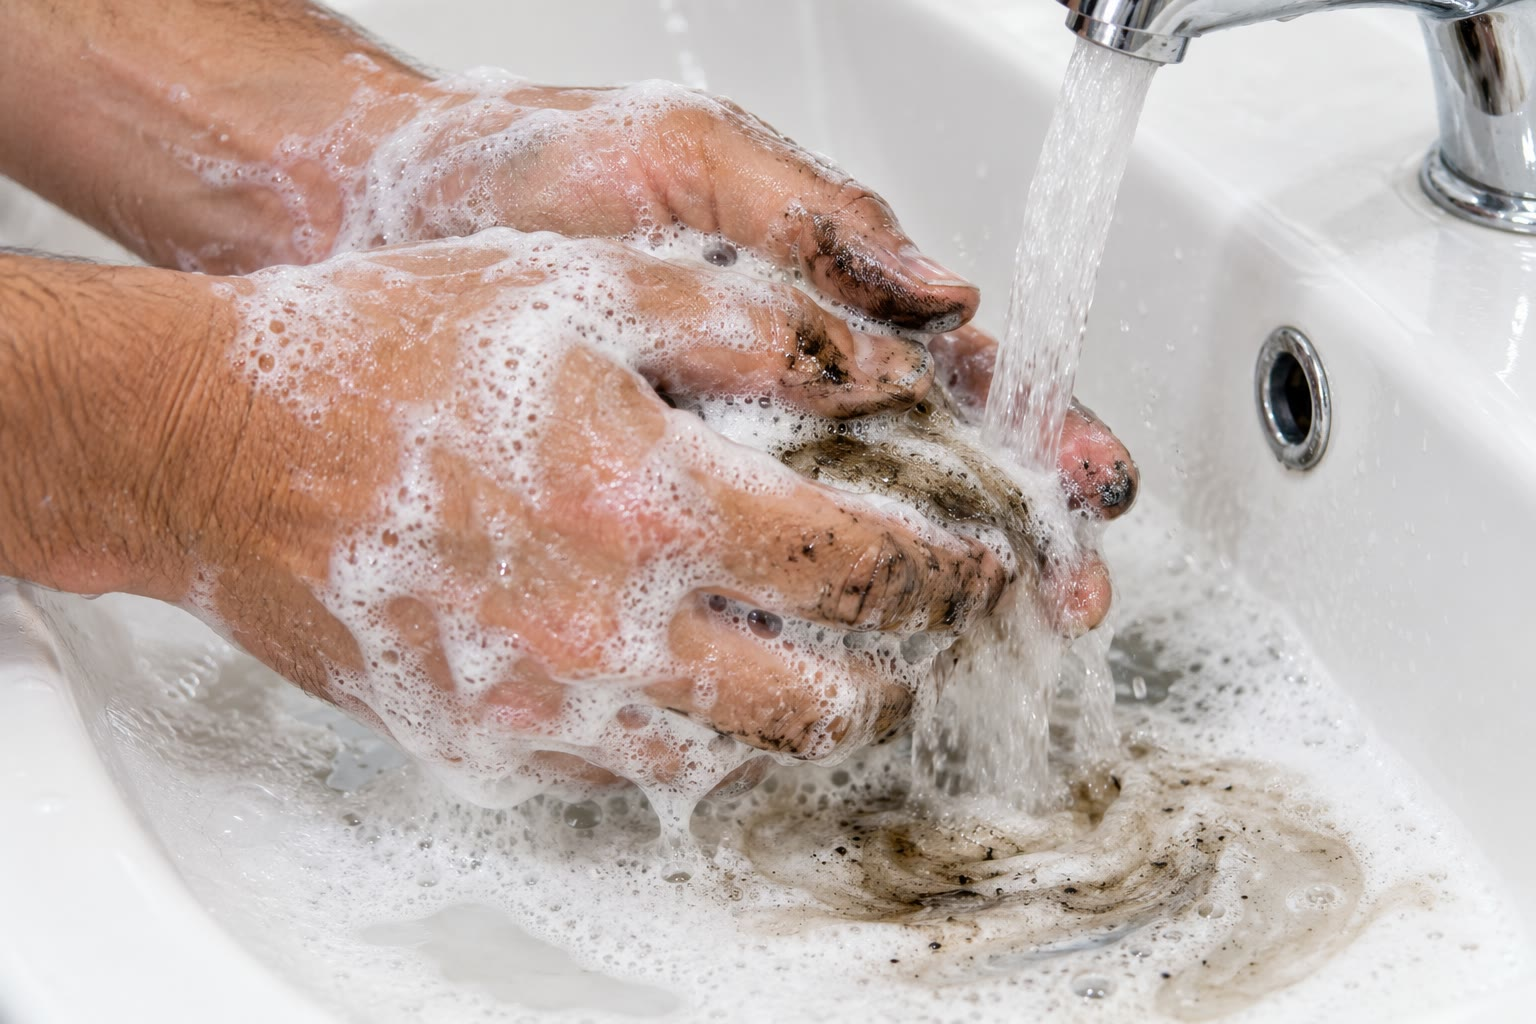
\includegraphics[width=0.48\linewidth]{images/book1/ai/g11-greasy-hands.jpg}

{\small Se laver les mains grasses~: le savon emporte la graisse dans des
\omterm{def:g11:dissolution:amphiphilic}{micelles}.}
\end{omfigure}

\begin{remark}[L'eau dure et le dépôt calcaire du savon]\label{rem:g11:dissolution:scum}
Une eau dure contient beaucoup d'\omterm{def:g9:ions:ion}{ions} calcium \ce{Ca^{2+}} et d'\omterm{def:g9:ions:ion}{ions}
magnésium \ce{Mg^{2+}}, dissous dans les roches qu'elle a traversées.
Avec les \omterm{def:g9:ions:ion}{ions} stéarate, ils forment un \omterm{def:g9:ions:precipitate}{précipité} (\cref{ch:g9:ions}), le
stéarate de calcium~:
\[
  \ce{2C17H35COO- + Ca^{2+} -> Ca(C17H35COO)2(s)} .
\]
Ce solide grisâtre est le dépôt qui cerne un lavabo, et chaque \omterm{def:g9:ions:ion}{ion} de
savon qui y est piégé est perdu pour le lavage~: dans une eau dure, le
savon mousse mal tant qu'on n'en a pas ajouté assez pour précipiter tout
le calcium.
\end{remark}

\begin{omfigure}
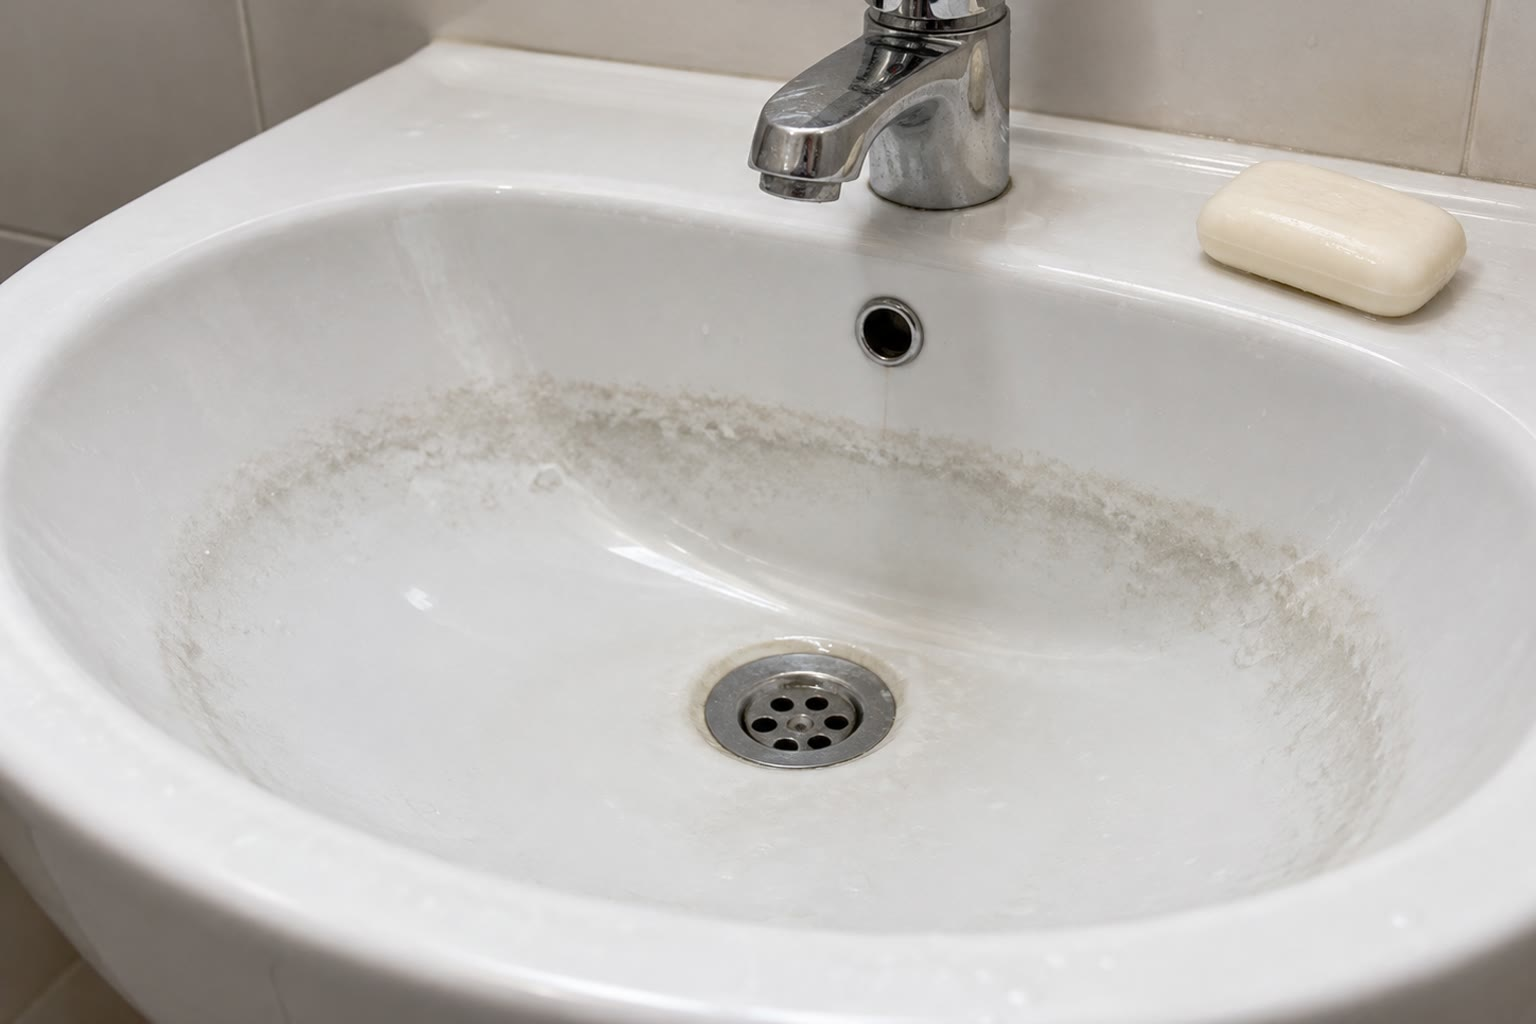
\includegraphics[width=0.45\linewidth]{images/book1/ai/g11-soap-scum.jpg}

{\small Un dépôt de savon dans un lavabo~: du stéarate de calcium,
\omterm{def:g9:ions:precipitate}{précipité} par une eau dure.}
\end{omfigure}

\section{Exercices}


\begin{exercise}[$\star$]\label{exo:g11:dissolution:1}
Écrire les équations de dissolution dans l'eau du chlorure de sodium
\ce{NaCl}, du chlorure de calcium \ce{CaCl2}, du sulfate de sodium
\ce{Na2SO4} et du chlorure d'aluminium \ce{AlCl3}.
\end{exercise}

\begin{exercise}[$\star$]\label{exo:g11:dissolution:2}
Une solution de sulfate de sodium a pour concentration
$c = \qty{0.050}{mol/L}$. Donner les concentrations des \omterm{def:g9:ions:ion}{ions} sodium et
des \omterm{def:g9:ions:ion}{ions} sulfate.
\end{exercise}

\begin{exercise}[$\star$]\label{exo:g11:dissolution:3}
Qu'appelle-t-on \omterm{def:g11:dissolution:solvation}{hydratation} d'un \omterm{def:g9:ions:ion}{ion}~? Quelle extrémité d'une \omterm{def:g7:atoms-and-molecules:molecule}{molécule}
d'eau est tournée vers un \omterm{def:g9:ions:ion}{cation}, laquelle vers un \omterm{def:g9:ions:ion}{anion}~? Pourquoi~?
\end{exercise}

\begin{exercise}[$\star$]\label{exo:g11:dissolution:4}
On dissout \qty{2.67}{g} de chlorure d'aluminium pour obtenir
\qty{200.0}{mL} de solution. Calculer la concentration de la solution et
celle de chaque \omterm{def:g9:ions:ion}{ion}.
\end{exercise}

\begin{exercise}[$\star$]\label{exo:g11:dissolution:5}
Indiquer si chaque partie de l'\omterm{def:g9:ions:ion}{ion} stéarate est \omterm{def:g11:dissolution:hydrophilic}{hydrophile} ou
\omterm{def:g11:dissolution:hydrophilic}{hydrophobe}, et dire pourquoi.
\end{exercise}

\begin{exercise}[$\star\star$]\label{exo:g11:dissolution:6}
Quel \omterm{def:g6:solutions-and-solubility:solute}{solvant}, l'eau ou le cyclohexane, choisirait-on pour dissoudre~: du
sel~; de la cire de bougie (longues chaînes hydrocarbonées)~; du sucre
(nombreux groupes \ce{O-H})~; du diiode~? Justifier chaque choix.
\end{exercise}

\begin{exercise}[$\star\star$]\label{exo:g11:dissolution:7}
L'éthanol \ce{CH3-CH2-OH} se \omterm{def:g6:pure-substances-and-mixtures:mixture}{mélange} à l'eau en toutes proportions,
mais l'hexane \ce{C6H14} ne se \omterm{def:g6:pure-substances-and-mixtures:mixture}{mélange} pas à l'eau. Expliquer.
\end{exercise}

\begin{exercise}[$\star\star$]\label{exo:g11:dissolution:8}
Observer la figure de la \omterm{def:g11:dissolution:amphiphilic}{micelle}. Pourquoi les queues sont-elles à
l'intérieur et les têtes à l'extérieur~? Pourquoi deux \omterm{def:g11:dissolution:amphiphilic}{micelles} ne
fusionnent-elles pas en une goutte de graisse plus grosse~?
\end{exercise}

\begin{exercise}[$\star\star$]\label{exo:g11:dissolution:9}
Un parfum végétal est dissous dans l'eau. Pour l'extraire, un chimiste
peut utiliser l'éthanol ou le cyclohexane. Lequel convient, et pourquoi
l'autre ne convient-il pas (penser à la miscibilité)~?
\end{exercise}

\begin{exercise}[$\star\star$]\label{exo:g11:dissolution:10}
Dans l'\omterm{def:g10:chemical-species:extraction}{extraction} du diiode, pourquoi la phase de cyclohexane est-elle
au-dessus~? Quelle phase évacue-t-on par le robinet~? Où se trouve le
diiode à la fin~?
\end{exercise}

\begin{exercise}[$\star\star$]\label{exo:g11:dissolution:11}
On agite une solution bleue de sulfate de cuivre avec du cyclohexane.
Que devient la couleur bleue~? Expliquer.
\end{exercise}

\begin{exercise}[$\star\star\star$]\label{exo:g11:dissolution:12}
Quelle masse de chlorure de calcium faut-il dissoudre pour obtenir
\qty{250.0}{mL} d'une solution dans laquelle
$[\ce{Cl-}] = \qty{0.300}{mol/L}$~?
\end{exercise}

\begin{exercise}[$\star\star\star$]\label{exo:g11:dissolution:13}
On trouve dans un échantillon d'eau de mer \qty{0.010}{mol/L} d'\omterm{def:g9:ions:ion}{ions}
calcium et \qty{0.053}{mol/L} d'\omterm{def:g9:ions:ion}{ions} magnésium. Expliquer pourquoi un
savon ordinaire mousse très mal dans l'eau de mer. Quelle masse de
stéarate de sodium serait précipitée par les seuls \omterm{def:g9:ions:ion}{ions} calcium d'un
litre d'eau de mer~?
\end{exercise}

\begin{exercise}[$\star\star\star$]\label{exo:g11:dissolution:14}
On \omterm{def:g6:pure-substances-and-mixtures:mixture}{mélange} \qty{100.0}{mL} de solution de chlorure de sodium à
\qty{0.20}{mol/L} avec \qty{100.0}{mL} de solution de chlorure de
calcium à \qty{0.10}{mol/L}. Aucun \omterm{def:g9:ions:precipitate}{précipité} ne se forme. Calculer les
concentrations de \ce{Na+}, \ce{Ca^{2+}} et \ce{Cl-} dans le \omterm{def:g6:pure-substances-and-mixtures:mixture}{mélange}, et
vérifier qu'il est neutre.
\end{exercise}

\begin{exercise}[$\star\star\star$]\label{exo:g11:dissolution:15}
% ledger: sol:I2-water, sol:I2-heptane, rho:heptane
Le diiode \omterm{def:g2:mixing-and-dissolving:dissolve}{se dissout} à raison d'environ \qty{0.3}{g} par litre d'eau et
de \qty{17}{g} par kilogramme d'heptane. L'heptane a une masse volumique
d'environ \qty{0.68}{kg/L}. Combien de fois plus de diiode un litre
d'heptane peut-il contenir qu'un litre d'eau~? Qu'est-ce que cela
signifie pour une \omterm{def:g10:chemical-species:extraction}{extraction}~?
\end{exercise}

\section{Problème~: le savon et l'eau dure}

\begin{problem}[{Problème du week-end --- combien de savon un bain d'eau
dure gaspille-t-il en dépôt~?}]
\label{pb:g11:dissolution:1}
% ledger: aw:Ca, aw:Mg, aw:C, aw:H, aw:O, aw:Na
Une eau du robinet contient \qty{120}{mg} d'\omterm{def:g9:ions:ion}{ions} calcium et \qty{24}{mg}
d'\omterm{def:g9:ions:ion}{ions} magnésium par litre. On remplit une baignoire de \qty{150}{L} de
cette eau, et le baigneur utilise un savon fait de stéarate de sodium,
\ce{C17H35COONa}.

\medskip
\noindent\textbf{Partie I --- Ce que contient l'eau.}
\begin{enumerate}
  \item D'où viennent les \omterm{def:g9:ions:ion}{ions} calcium et magnésium de l'eau du
        robinet~?
  \item Calculer les \omterm{def:g10:concentration-and-dilution:molar-concentration}{concentrations molaires} des \omterm{def:g9:ions:ion}{ions} calcium et des
        \omterm{def:g9:ions:ion}{ions} magnésium.
  \item Les \omterm{def:g9:ions:ion}{ions} calcium sont accompagnés d'\omterm{def:g9:ions:ion}{ions} hydrogénocarbonate,
        \ce{HCO3-}, comme si l'on avait dissous de l'hydrogénocarbonate de
        calcium \ce{Ca(HCO3)2}. Écrire cette équation de dissolution, et
        en déduire la concentration des \omterm{def:g9:ions:ion}{ions} hydrogénocarbonate qui
        accompagnent le calcium.
  \item Quelle quantité d'\omterm{def:g9:ions:ion}{ions} calcium la baignoire contient-elle~?
\end{enumerate}

\medskip
\noindent\textbf{Partie II --- Le savon.}
\begin{enumerate}[resume]
  \item Calculer la \omterm{def:g10:the-mole:molar-mass}{masse molaire} du stéarate de sodium.
  \item Écrire son équation de dissolution dans l'eau.
  \item Quelle partie de l'\omterm{def:g9:ions:ion}{ion} stéarate est \omterm{def:g11:dissolution:hydrophilic}{hydrophile}, quelle partie
        \omterm{def:g11:dissolution:hydrophilic}{hydrophobe}~? Pourquoi le dit-on \omterm{def:g11:dissolution:amphiphilic}{amphiphile}~?
  \item Décrire une \omterm{def:g11:dissolution:amphiphilic}{micelle}, et expliquer comment elle élimine la
        graisse de la peau.
  \item Pourquoi faut-il dissoudre le savon dans l'eau, et non dans
        l'huile, pour se laver~?
\end{enumerate}

\medskip
\noindent\textbf{Partie III --- Le dépôt.}
\begin{enumerate}[resume]
  \item Écrire l'équation de la \omterm{def:g9:ions:precipitate}{précipitation} du stéarate de calcium.
        Vérifier qu'elle est ajustée en charges.
  \item Remplir le \omterm{def:g10:reaction-progress-table:extent}{tableau d'avancement} pour \qty{1.00}{L} d'eau du
        robinet et un excès d'\omterm{def:g9:ions:ion}{ions} stéarate. Quel \omterm{def:g7:chemical-reactions:reactant}{réactif} est
        limitant~?
  \item Quelle quantité d'\omterm{def:g9:ions:ion}{ions} stéarate est perdue par litre au profit
        du calcium~?
  \item Calculer la \omterm{def:g10:the-mole:molar-mass}{masse molaire} du stéarate de calcium, et la masse de
        dépôt formée par litre.
  \item Le stéarate de magnésium précipite de la même façon. Quelle
        quantité de stéarate les \omterm{def:g9:ions:ion}{ions} magnésium accaparent-ils par
        litre~?
\end{enumerate}

\medskip
\noindent\textbf{Partie IV --- Le bain.}
\begin{enumerate}[resume]
  \item Quelle quantité d'\omterm{def:g9:ions:ion}{ions} stéarate le calcium de toute la baignoire
        précipite-t-il~?
  \item À quelle masse de savon cela correspond-il~?
  \item En ajoutant le magnésium, quelle masse de savon est gaspillée au
        total~?
  \item Un pain de savon pèse environ \qty{100}{g}. Combien de pains le
        calcium seul accapare-t-il~?
  \item Donner la réponse finale~: quelle masse de savon le calcium d'un
        bain de \qty{150}{L} de cette eau gaspille-t-il en dépôt~?
\end{enumerate}
\end{problem}
